% !Mode:: "TeX:UTF-8"
\chapter{模型实现以及结果分析}
本节通过构造一个社交网络用户影响力分析模型来实现本次的课程设计。将在算法原理的基础上详细介绍本次课设包含的处理模块,最终将所建立模型的与实际情况作比较进行误差分析。
\section{抓取到的部分微博数据}
\begin{figure}[h]
	\centering
	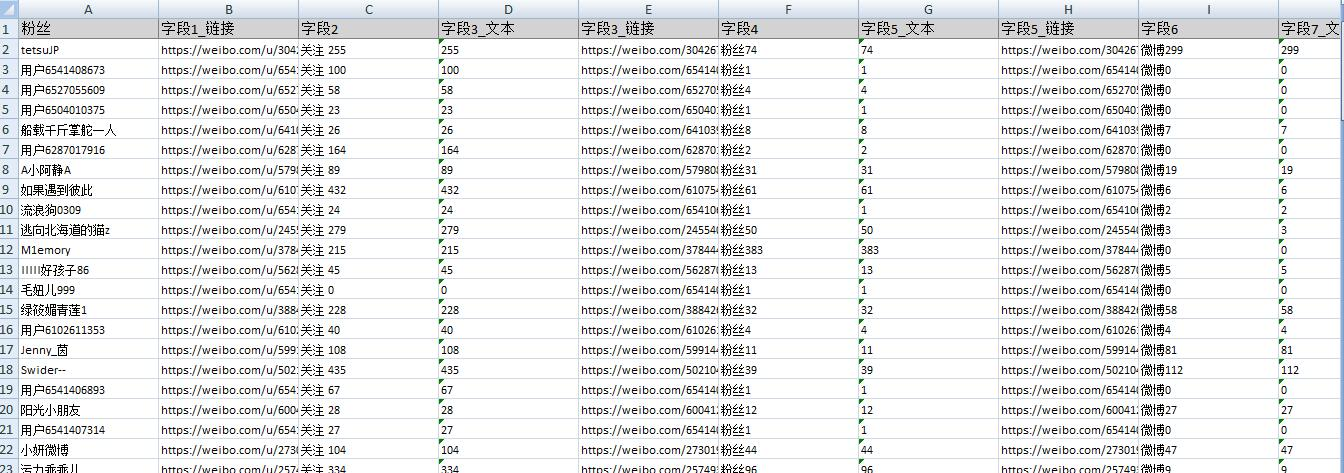
\includegraphics[scale=0.5]{figures/3.png}
	\caption{部分微博数据}
	\label{fig:1}
\end{figure}

\section{社交网络用户行为分析系统IPO图}
IPO图为输入处理加工图的建成,用来说明输入数据,对输入数据的数据加工过程,以及输出数据。本次实验所涉及到的IPO图如图4.2所示
\begin{figure}[h]
	\centering
	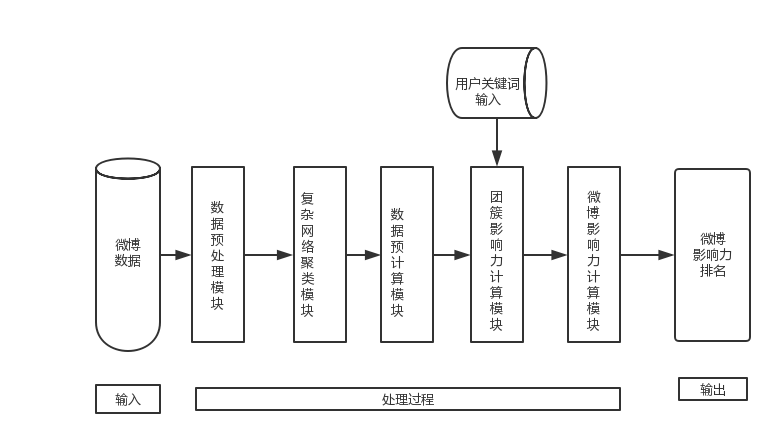
\includegraphics[scale=0.5]{figures/4.png}
	\caption{社交网络用户行为分析系统}
	\label{fig:1}
\end{figure}
\begin{enumerate}[(1)]
\item 数据预处理模块
\item 对复杂网络进行聚类分析模块
\item 对数据进行与计算模块
\item 团簇影响力的计算
\item 微博影响力的计算。输出数据为聚类中度的出度,入度分布,度中心度分布,距离中心分布。
\end{enumerate}

\section{社交网络影响力分析系统的实现}
\subsection{数据预处理模块}
该模块的主要功能是对爬取到的微博数据进行预处理,主要可分为两部分,如图4.3:
\begin{enumerate}[(1)]
	\item 剔除粉丝数目为零的用户
	\item 剔除僵尸粉
\end{enumerate}
\begin{figure}[h]
	\centering
	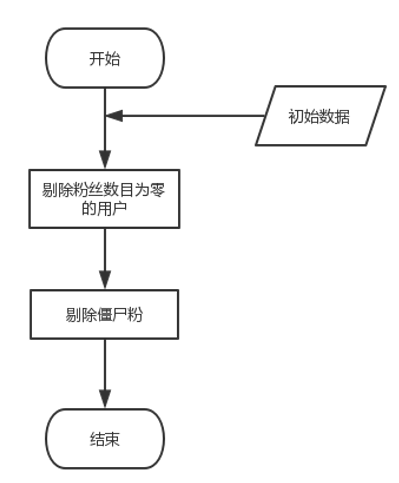
\includegraphics[scale=0.5]{figures/5.png}
	\caption{数据预处理流程图}
	\label{fig:1}
\end{figure}

\subsection{社交网络聚类模块}
社交网络聚类模块对上一模块的输出数据进行聚类处理。该部分通过微博连接关系构建社交网络,并且使用改进过的GN算法把社交网络分解为多个相互联系紧密且可以独立研究的团簇。模块的具体计算流如图4.4:
\begin{figure}[h]
	\centering
	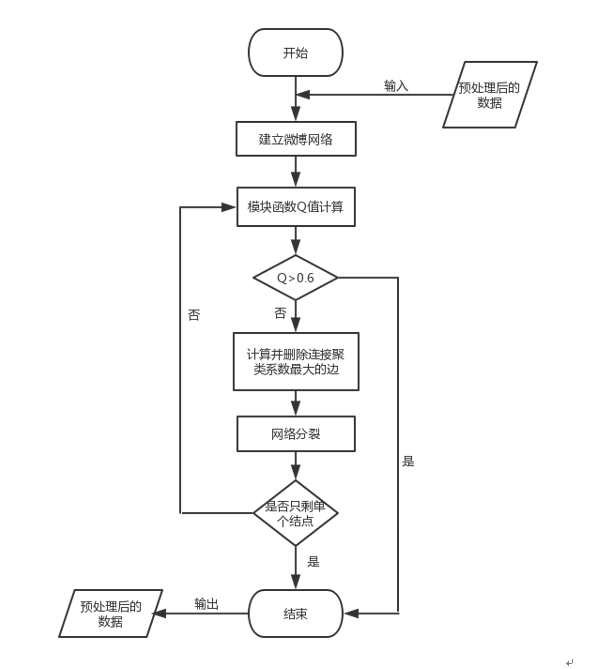
\includegraphics[scale=0.5]{figures/6.png}
	\caption{复杂网络聚类模块流程图}
	\label{fig:1}
\end{figure}
数据经过该模块处理完成之后,所有的社交网络用户都将拥有一个标示用于指示用户所属的团簇。

\subsection{数据预计算模块}
在实际计算微博影响力的时候,采用的是用迭代的方法并结合pagerank算法,导致计算较为缓慢。但是其中涉及到的部分数据,例如用户的平均粉丝数,平均微博数等,可以先将这几个参数进行预计算并将结果存入数据库之中,便可以提高系统的计算实时性。

\subsection{团簇影响力计算模块}
此部分的计算模块是对上一步已经进行完毕聚类的团簇进行影响力计算,以此来作为微博影响力计算的参数。如图4.5

\begin{figure}[h]
	\centering
	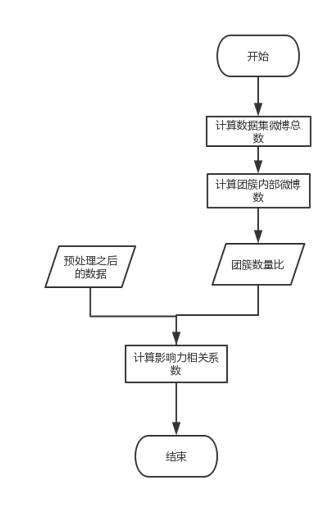
\includegraphics[scale=0.5]{figures/7.png}
	\caption{团簇影响力计算模块流程图}
	\label{fig:1}
\end{figure}

\subsection{社交网络用户影响力计算模块}
微博用户影响力计算模块是在前几个已经完成的模块基础上对最终的社交网络影响力进行计算,由于PR值以及团簇内部已经被计算。故在此模块计算之后即可做出最终的社交用户影响力数据相关度分布。其计算模块流如图4.6
\begin{figure}[h]
	\centering
	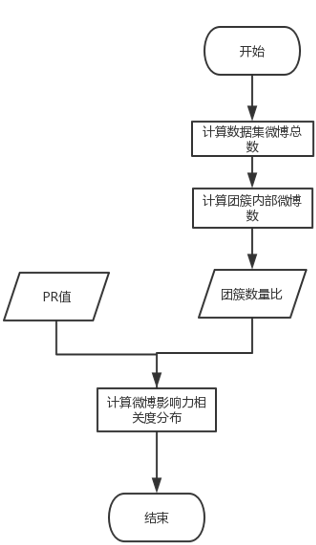
\includegraphics[scale=0.5]{figures/8.png}
	\caption{微博影响力计算模块流程图}
	\label{fig:1}
\end{figure}

\section{实验结果及分析}
对模型的评价在于对利用多种方式对微博偏好影响力计算的实时性进行评估,对其进行横向对比。图4.7-图4.12分别为网络节点中的度性能坐标分析图。


\begin{figure}[h]
	\centering
	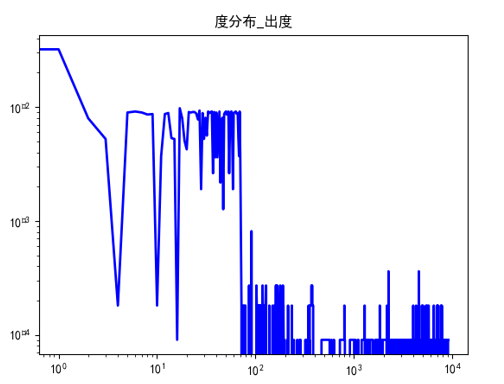
\includegraphics[scale=0.5]{figures/9.png}
	\caption{度分布-出度}
	\label{fig:1}
\end{figure}

\begin{figure}[h]
	\centering
	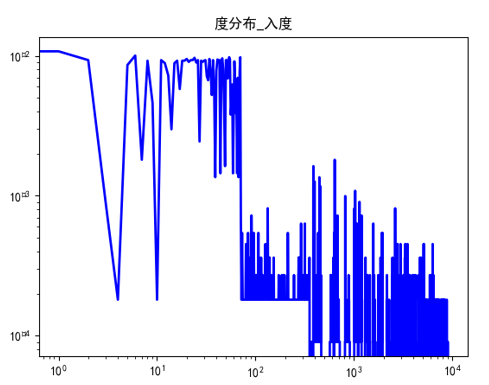
\includegraphics[scale=0.5]{figures/10.png}
	\caption{度分布-入度}
	\label{fig:1}
\end{figure}

\begin{figure}[h]
	\centering
	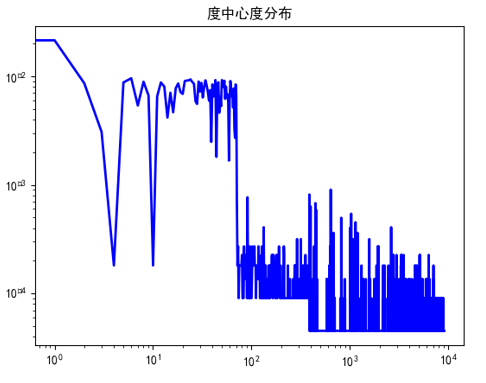
\includegraphics[scale=0.5]{figures/11.png}
	\caption{度中心度分布}
	\label{fig:1}
\end{figure}

\begin{figure}[h]
	\centering
	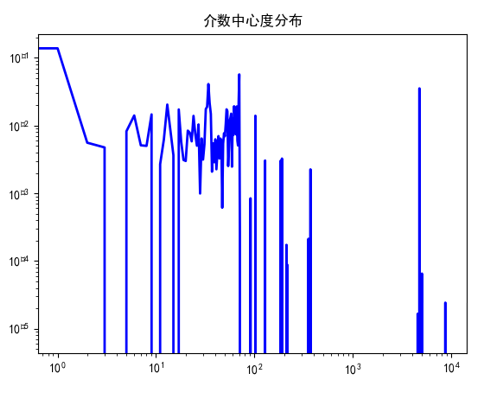
\includegraphics[scale=0.5]{figures/12.png}
	\caption{介数中心度分布}
	\label{fig:1}
\end{figure}

\begin{figure}[h]
	\centering
	
\includegraphics[scale=0.5]{figures/13.png}
	\caption{距离中心度分布}
	\label{fig:1}
\end{figure}

\begin{figure}[h]
	\centering
	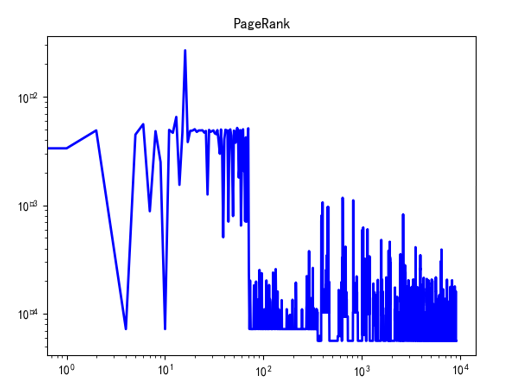
\includegraphics[scale=0.5]{figures/14.png}
	\caption{page rank分布}
	\label{fig:1}
\end{figure}

从这些图可以看出,节点的频次数目随着出入度的增加而减少,节点出入度越大,其所对应的中心距离度越大。且随着节点出入度的增加,各类数值频次趋于稳定,在数据集增加到为10\^2为级别时,所得出结论逐渐稳定。其中pagerank算法由于其参数方面对用户关键词的计算度量较少因此结果比较不稳定。
\par
在社交网络中,当一个用户节点出入度以及距离中心度等越大时,其用户影响力越大。且在社交网络总体之中此类用户节点所占比例较小。 













